% !TeX root = Otimizacao.tex
% !TeX encoding = UTF-8
% !TeX spellcheck = pt_BR
% !TeX program = pdflatex
\section{Conjuntos convexos}

\subsection{Conjuntos afins e convexos}

\begin{frame}{Conjuntos afins}
  \begin{columns}
    \begin{column}{0.63\linewidth}
      \begin{itemize}\addtolength{\itemsep}{\baselineskip}
        \item Linha e segmentos
        \begin{itemize}
        \item Sejam os pontos $ \vtX_1, \vtX_2 \in \fdR^n $ com $ \vtX_1 \neq \vtX_2 $ \ding{220} pontos $ \vtY $ da
          forma $ \vtY = \theta\vtX_1 + (1-\theta)\vtX_2 $ com $ \theta \in \fdR$, $ 0 \leq \theta \leq 1 $, formam um
          segmento fechado ligando $ \vtX_1 $ a $ \vtX_2 $
          \item Representando $ \vtY = \vtX_2 + \theta(\vtX_1 - \vtX_2) $ \ding{220} Ponto base $ \vtX_2 $ e direção $ 
          (\vtX_1 - \vtX_2) $ apontando de $ \vtX_2 $ para $ \vtX_1 $ e escalonada por $ \theta $
        \end{itemize}
        
        \item Conjuntos afins 
        \begin{itemize}
          \item Um conjunto $ \fdA\subset \fdR^n$ é afim \ding{220} para qualquer $ \vtX_1, \vtX_2 \in \fdA\subset 
          \fdR$ e $ \theta \in \fdR $, o segmento de reta $ \vtY =  \theta\vtX_1 + (1-\theta)\vtX_2 \in \fdA$
          \item Combinação afim \ding{220} $ \vtY = \theta_1 \vtX_1 + \theta_2 \vtX_2 + \ldots + \theta_k \vtX_k \in 
          \fdA\subset \fdR $, com $ \theta_1 + \theta_2 + \ldots + \theta_k = 1 $
        \end{itemize}
      \end{itemize}
    \end{column}
    \begin{column}{0.33\linewidth}
      \centering
      \begin{tikzpicture}[thick,scale=0.8]
        \draw[help lines] (0,0) grid (5,4);
        \coordinate (x1) at (1,1);
        \node at (x1) [above] {$ \vtX_1 $};
        \coordinate (x2) at (4,3);
        \node at (x2) [above] {$ \vtX_2 $};
        \draw[black] (x1) -- (x2);
        \fill[black] ($(x1)$) circle (2pt);
        \fill[black] ($(x2)$) circle (2pt);
        \fill[red] ($(x1)!.4!(x2)$) circle (2pt);
        \node at ($(x1)!.4!(x2)$) [below right] {$ \vtY $};
      \end{tikzpicture}
      
      \vspace*{\baselineskip}
      
      \begin{tikzpicture}[thick,scale=0.8]
        \draw[help lines] (0,0) grid (5,4);
        \coordinate (x1) at (1,1);
        \node at (x1) [above] {$ \vtX_1 $};
        \coordinate (x2) at (4,3);
        \node at (x2) [above] {$ \vtX_2 $};
        \draw[red] ($(x1)!-.3!(x2)$) -- ($(x1)!1.3!(x2)$);
        \draw[black] (x1) -- (x2);
        \fill[black] ($(x1)$) circle (2pt);
        \fill[black] ($(x2)$) circle (2pt);
        \fill[red] ($(x1)!.4!(x2)$) circle (2pt);
        \node at ($(x1)!.4!(x2)$) [below right] {$ \vtY $};
      \end{tikzpicture}
    \end{column}
  \end{columns}
\end{frame}

\begin{frame}{Conjuntos convexos}
  \begin{columns}
    \begin{column}{0.63\linewidth}
      \begin{itemize}\addtolength{\itemsep}{\baselineskip}
        \item Conjuntos convexos
        \begin{itemize}
        \item Um conjunto $ \fdA \subset \fdR^n$ é convexo caso um segmento entre $\vtX_{1}, \vtX_{2} \in \fdA$ e $ 0
          \leq \theta \leq 1 $, pertença a $ \fdA$, ou seja, $ \theta \vtX_{1}+(1-\theta) \vtX_{2} \in \fdA$
          \item Em termos geométricos, um conjunto convexo é um conjunto sem buracos ou reentrâncias
        \end{itemize}
        
        \item Invólucro convexo (\textit{convex hull})
        \begin{itemize}
          \item Dado um conjunto $ \fdA$, o invólucro convexo de $ \fdA $ é o menor conjunto convexo que engloba $ \fdA 
          $, sendo denotado por $ \Conv{\fdA} = \{ \theta_{1} \vtX_{1} + \cdots + \theta_{k} \vtX_{k} \mid \vtX_{i} \in 
          \fdA, \theta_{i} \geq 0, i=1, \cdots, k, \theta_{1} + \cdots + \theta_{k} = 1\} $
        \end{itemize}
      \end{itemize}
    \end{column}
    \begin{column}{0.33\linewidth}
      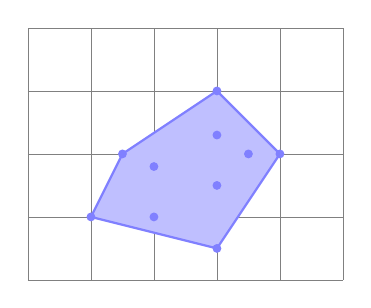
\begin{tikzpicture}[thick,scale=0.8]
        \draw[help lines] (0,0) grid (5,4);
        \coordinate (x1) at (1,1);
        \coordinate (x2) at (3,0.5);
        \coordinate (x3) at (4,2);
        \coordinate (x4) at (3,3);
        \coordinate (x5) at (1.5,2);
        \path[draw,color=Blue!50,fill=Blue!25] (x1) -- (x2) -- (x3) -- (x4) -- (x5) -- cycle;
        \fill[draw=none,fill=Blue!50] (x1) circle (2pt);
        \fill[draw=none,fill=Blue!50] (x2) circle (2pt);
        \fill[draw=none,fill=Blue!50] (x3) circle (2pt);
        \fill[draw=none,fill=Blue!50] (x4) circle (2pt);
        \fill[draw=none,fill=Blue!50] (x5) circle (2pt);
        \fill[draw=none,fill=Blue!50] (2,1) circle (2pt);
        \fill[draw=none,fill=Blue!50] (3,1.5) circle (2pt);
        \fill[draw=none,fill=Blue!50] (3.5,2) circle (2pt);
        \fill[draw=none,fill=Blue!50] (2, 1.8) circle (2pt);
        \fill[draw=none,fill=Blue!50] (3, 2.3) circle (2pt);
      \end{tikzpicture}

      \vspace*{\baselineskip}

      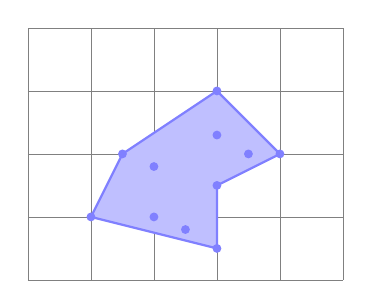
\begin{tikzpicture}[thick,scale=0.8]
        \draw[help lines] (0,0) grid (5,4);
        \coordinate (x1) at (1,1);
        \coordinate (x2) at (3,0.5);
        \coordinate (x3) at (3,1.5);
        \coordinate (x4) at (4,2);
        \coordinate (x5) at (3,3);
        \coordinate (x6) at (1.5,2);
        \path[draw,color=Blue!50,fill=Blue!25] (x1) -- (x2) -- (x3) -- (x4) -- (x5) -- (x6) -- cycle;
        \fill[draw=none,fill=Blue!50] (x1) circle (2pt);
        \fill[draw=none,fill=Blue!50] (x2) circle (2pt);
        \fill[draw=none,fill=Blue!50] (x3) circle (2pt);
        \fill[draw=none,fill=Blue!50] (x4) circle (2pt);
        \fill[draw=none,fill=Blue!50] (x5) circle (2pt);
        \fill[draw=none,fill=Blue!50] (x6) circle (2pt);
        \fill[draw=none,fill=Blue!50] (2,1) circle (2pt);
        \fill[draw=none,fill=Blue!50] (2.5,0.8) circle (2pt);
        \fill[draw=none,fill=Blue!50] (3.5,2) circle (2pt);
        \fill[draw=none,fill=Blue!50] (2, 1.8) circle (2pt);
        \fill[draw=none,fill=Blue!50] (3, 2.3) circle (2pt);
      \end{tikzpicture}
    \end{column}
  \end{columns}
\end{frame}

\subsection{Operações sobre conjuntos que preservam convexidade}

\begin{frame}{Operações sobre conjuntos que preservam convexidade}
  \vspace*{-0.5\baselineskip}
  \begin{itemize}\footnotesize\setlength{\AuxWidth}{\widthof{Multiplicação por escalar}}
    \item \makebox[\AuxWidth][l]{Interseção} \ding{220} se $ \fdA_{\alpha}$ é convexo para todo $\alpha \in \fdR$, então %
    \begin{equation}\label{eq_oper_inter}
      \bigcap_{\alpha \in \fdR} \fdA_{\alpha} \quad \quad \quad \text{também é convexo}
    \end{equation} %

    \item \makebox[\AuxWidth][l]{Multiplicação por escalar} \ding{220} se $ \fdA \subseteq \fdR^n$ é convexo e $\alpha \in \fdR$, então %
    \begin{equation}\label{eq_oper_escalar}
      \alpha \fdA = \{ \alpha \vtX \mid \vtX \in \fdA \} \quad \quad \quad \text{também é convexo}
    \end{equation} 
    
    \item \makebox[\AuxWidth][l]{Translação} \ding{220} se $ \fdA \subseteq \fdR^n$ é convexo e $\vtAlpha \in \fdR^n$, então %
    \begin{equation}\label{eq_oper_trans}
      \fdA + \vtAlpha = \{ \vtX + \vtAlpha \mid \vtX \in \fdA \} \quad \quad \quad \text{também é convexo}
    \end{equation} %

    \item \makebox[\AuxWidth][l]{Soma} \ding{220} se $\fdA_{1}$ e $\fdA_{2}$ são convexos, então %
    \begin{equation}\label{eq_oper_soma}
      \fdA_{1} + \fdA_{2} = \{ \vtX + \vtY \mid \vtX \in \fdA_{1}, \vtY \in \fdA_{2}\} \quad \quad \quad \text{também é convexo}
    \end{equation} %
      
    \item \makebox[\AuxWidth][l]{Produto cartesiano} \ding{220} se $\fdA_{1}$ e $\fdA_{2}$ são convexos, então %
    \begin{equation}\label{eq_oper_pcart}
      \fdA_{1} \times \fdA_{2} = \{ (\vtX, \vtY) \mid \vtX \in \fdA_{1}, \vtY \in \fdA_{2}\}\quad \quad \quad \text{também é convexo}
    \end{equation} %
  \end{itemize}
\end{frame}

\subsection{Hiperplanos, cones e desigualdades generalizadas}

\begin{frame}{Hiperplanos, cones e desigualdades generalizadas}
  \begin{columns}
    \begin{column}{0.48\linewidth}
      \begin{itemize}
        \item Hiperplano \ding{220} conjunto de pontos, podendo ser escrito como
        \begin{equation}\label{eq_hiperplano}
        \{ \vtX \mid \Transp{\vtA}(\vtX-\vtX_{0}) = 0) \}
        \end{equation}
        onde $ \vtA \in \fdR^n$, $ \vtA \neq \vtZero$, e $\vtX_{0}$ determina o offset do hiperplano. Um hiperplano divide o espaço em dois semi-espaços
        
        \item Semi-espaço \ding{220} conjunto da forma  
        \begin{equation}\label{eq_halfspace}
        \{ \vtX \mid \Transp{\vtA}(\vtX-\vtX_{0}) \leq 0) \}
        \end{equation}
        onde $ \vtA \in \fdR^n$, $ \vtA \neq \vtZero$
      \end{itemize} 
    \end{column}

    \hfill

    \begin{column}{0.48\linewidth}
      % TODO: Adicionar figuras
      \begin{block}{TODO}
        Adicionar figuras
      \end{block}
    \end{column}
  \end{columns}
\end{frame}

\begin{frame}{Hiperplanos, cones e desigualdades generalizadas}
  \begin{columns}
    \begin{column}{0.48\linewidth}
      \begin{itemize}
        \item Cone é conjunto de pontos tais que $ \forall \vtX \in \fdA \subset \fdR^n$ e $ \theta \geq 0, \theta \in \fdR_{+}$
        \begin{equation}\label{eq_cone}
          \theta \vtX \in \fdA, \forall \vtX \in \fdA
        \end{equation}
       
        \item Cone Convexo é um conjunto que é simultaneamente um cone e convexo, ou seja, para qualquer $\vtX_{1}, \vtX_{2} \in \fdA \subset \fdR^n$ e $ \theta_{1}, \theta_{2} \geq 0, \theta_1$
        \begin{equation}\label{eq_cone_conv}
          \theta_{1} \vtX_{1} + \theta_{2} \vtX_{2} \in \fdA
        \end{equation}
      \end{itemize}
    \end{column}

    \hfill

    \begin{column}{0.48\linewidth}
      % TODO: Adicionar figuras
      \begin{block}{TODO}
        Adicionar figuras
      \end{block}
    \end{column}
  \end{columns}
\end{frame}

\begin{frame}{Conjuntos Convexos}
  \begin{columns}
    \begin{column}{0.48\linewidth}
      \begin{itemize}
        \item A bola Euclidiana com o centro em $\vtX_{c}$ e raio $r$ é representada por
        \begin{equation}\label{eq_ball}
          B(\vtX_{c}, r) = \{ \vtX_{c} + r\vtU \mid \NormTwo{\vtU} \leq 1 \}
        \end{equation}
        
        \item O elipsoide com o centro em $\vtX_{c}$ é um conjunto representado na forma
        \begin{equation}\label{eq_elipsoide}
          \calE = \{ \vtX \mid \Transp{(\vtX-\vtX_{c})} \Inv{\mtP} (\vtX-\vtX_{c}) \leq 1) \}
        \end{equation}
        onde $ \mtP \in \fdA \subset \fdS^n_{++}$, ou seja, $ \mtP $ é uma matriz simétrica positiva definida
      \end{itemize}
    \end{column}

    \hfill

    \begin{column}{0.48\linewidth}
      % TODO: Adicionar figuras
      \begin{block}{TODO}
        Adicionar figuras
      \end{block}
    \end{column}
  \end{columns}
\end{frame}

\begin{frame}{Conjuntos Convexos}
  \begin{itemize}
    \item Poliedro
    \begin{itemize}
      \item O poliedro é definido como um conjunto de igualdades lineares e inequações.
      
      \begin{equation}\label{eq_poliedro}
      A x \preceq b, C x = d
      \end{equation}
      onde $\preceq$ é o símbolo que representa desiguadade componente a componente entre vetores.
      
      \item Dessa forma, a representação do poliedro pode escrita como: 
      
      \begin{equation}\label{eq_poliedro_2}
      P = \{ x \mid A x \preceq b, C x = d \}
      \end{equation}
    \end{itemize}
    
  \end{itemize}
\end{frame}


\begin{frame}{Conjuntos Convexos}
  
  \begin{itemize}
    \item Norma da Bola com centro $x_{c}$ e raio $r$ é representado por:
    
    \begin{equation}\label{eq_norm_ball}
    \{ x \mid \Norm{x-x_c} \leq r \}
    \end{equation}
    onde $\Norm{\cdot}$ é a norma.
    
    \item A norma do cone pode ser definido como:
    
    \begin{equation}\label{eq_norm_cone}
    \{ (x,t) \in  \fdR^n+1 \mid \Norm{x} \leq t \}
    \end{equation}
  \end{itemize}
  
\end{frame}



\begin{frame}{Conjuntos Convexos}
  
  \begin{itemize}
    \item PSD (Cone positivo semidefinido) é um cone formado a parti das matrizes positivas semidefinidas que utiliza a notação:
    
    \begin{equation}\label{eq_psd}
    \fdA^n_+ = \{ X \in \fdA^n \mid X \succ 0 \}
    \end{equation}
    onde $\fdA^n$ denota o conjunto de matrizes simetricas. Dessa forma o conjunto $\fdA^n_+$ é um cone positivo 
    semidefinido, se $ \theta_{1}, \theta_{2} \geqslant 0$ e $A, B \in \fdA^n_+$, assim $ \theta_{1} A + \theta_{2} B 
    \in \fdA^n_+$.  
  \end{itemize}
\end{frame}



\begin{frame}{Conjuntos Convexos}
  
  \begin{itemize} 
    \item Desigualdade generalizadas
    \begin{itemize}
      \item Um cone pode ser usado para definir a desigualdade generalizada, que é similar a relação de ordem apresentada em $\fdR$. Desta forma, para um cone $ K $ onde $ K \subseteq \fdR^n$, as desigualdades não estritas e estritas $ \preceq_{K}$ e $\prec_{K}$, respectivamente são definidas da seguinte maneira:
      
      \begin{subequations}
        \begin{align}
        x \preceq_{K} y \Leftrightarrow y - x \in K\\
        x \prec_{K} y \Leftrightarrow y - x \in \textbf{int(}K\textbf{)}
        \end{align}
      \end{subequations}
      
      onde $\textbf{int($K$)}$ representa o interior do conjunto $K$.
      
      \item Propriedades
      \begin{itemize}
        \item Se $x \preceq_{K} y$ e $u \preceq_{K} v$, então $ x + u \preceq_{K} y + v$
        \item  Se $x \preceq_{K} y$ e $y \preceq_{K} u$, então $ x \preceq_{K} u$
        \item  Se $x \preceq_{K} y$ e $y \preceq_{K} x$, então $ x = y$
        \item  Se $x \prec_{K} y$ e $u \preceq_{K} v$, então $ x + u \prec_{K} y + v$
      \end{itemize}
      
    \end{itemize}
    
  \end{itemize}
\end{frame}

\section{Propriedades básicas}

\subsection{Propriedades básicas e exemplos}

\begin{frame}{Propriedades básicas}
  \begin{itemize}
    \item Uma função $f: \bbR^n \rightarrow \bbR^n$ é convexa somente se o domínio de $f$ ($\dom f$) for convexo e 
    $\forall x, y \in \dom f$, e $0 \leq \theta \leq 1$ \eqref{eq:condConvexidade} for verdade.
    \begin{equation}
      f(\theta x + (1-\theta) y) \leq \theta f(x) + (1-\theta) f(y)
      \label{eq:condConvexidade}
    \end{equation}
    \item Observando a condição \eqref{eq:condConvexidade}, temos que em uma função $f(\cdot)$ convexa, qualquer 
    segmento de reta entre os pontos $(x, f(x))$ e $(y, f(y))$ estará acima de $f(\cdot)$ entre os valores $x$ e $y$, 
    como mostrado na figura abaixo.
    \begin{figure}
      \centering
%      \includegraphics[scale=0.2]{convexFunction}
    \end{figure}
  \end{itemize}
\end{frame}

\begin{frame}
  \frametitle{Propriedades básicas}
  \begin{itemize}
    \item Dizemos que uma função $f(\cdot)$ é estritamente convexa se a desigualdade ocorrer sempre para $0 < \theta < 
    1$ e $x \neq y$, ou seja,
    \begin{equation}
      f(\theta x + (1-\theta) y) < \theta f(x) + (1-\theta) f(y)
      \label{eq:condConvexidadeEstrita}
    \end{equation}
    \item Define-se uma função $f(\cdot)$ como côncava, se $-f(\cdot)$ for convexa.
    \item Funções afins são convexas e côncavas, visto que
    \begin{equation}
      f(\theta x + (1-\theta) y) = \theta f(x) + (1-\theta) f(y)
      \label{eq:condFuncaoAfim}
    \end{equation}
    para $0 \leq \theta \leq 1$.
  \end{itemize}
\end{frame}

\begin{frame}
  \frametitle{Propriedades básicas}
  \begin{itemize}
    \item Uma função $f(\cdot)$ é convexa se e somente se ela é convexa quando restrita a qualquer linha que intercepta 
    seu domínio. Ou seja, $f(x)$ é convexa se e somente se para todo $x \in \dom f$ e para todo $v$, a função $g(t) = 
    f(x + tv)$ é convexa no domínio $\{t | x + tv \in \dom f\}$.
    \item Esta propriedade é muito importante, pois pode-se avaliar a convexidade de uma função, restringindo-a a uma 
    linha.
  \end{itemize}
\end{frame}

\begin{frame}
  \frametitle{Extensão}
  \begin{itemize}
    \item As vezes é conveniente que o domínio da função $f(\cdot)$ seja estendido para todo $\bbR^n$, atribuindo o 
    valor $\infty$ para $f(x)$ quando $x \notin \dom f$.
    \item Assim, a extensão de $f(x)$, $\tilde{f}: \bbR^n \rightarrow \bbR \cup \infty$ é definida como:
    \begin{equation}
      \tilde{f}(x) = \left\{\begin{array}{ll}
        f(x) & x \in \dom f \\
        \infty & x \notin \dom f
      \end{array} \right.
    \end{equation}
    \item Essa extensão é útil pelo fato de simplificar a notação e de não haver a necessidade de se explicitar o seu 
    domínio.
    \item De modo análogo, podemos estender funções côncavas adicionando $-\infty$ a seu domínio.
  \end{itemize}
\end{frame}

\begin{frame}{Condições de primeira ordem}
  \begin{itemize}
    \item Seja $f(\cdot)$ uma função diferenciável, então $f(\cdot)$ é convexo se e somente se o $\dom f$ for convexo e 
    \begin{equation}
      f(y) \geq f(x) + \nabla \Transp{f(x)} (y-x) \,\,\,\,\,\, \forall x,y \in \dom f
      \label{eq:condPrimeiraOrdem}
    \end{equation} 
    \item Note que o segundo termo de \eqref{eq:condPrimeiraOrdem} é uma função afim em relação a $y$ e que é igual a 
    aproximação de primeira ordem de Taylor de $f(y)$ em torno de $x$.
    \begin{figure}
      \centering
%      \includegraphics[scale=0.3]{firstOrderCondition}
    \end{figure}
  \end{itemize}
\end{frame}

\begin{frame}{Condições de primeira ordem}
  \begin{itemize}
    \item Assim, se a aproximação de primeira ordem de Taylor de uma função sempre representar um subestimador global, 
    a função $f(\cdot)$ é convexa.
    \item De \eqref{eq:condPrimeiraOrdem}, podemos ver que a partir da informação local ($x$ e $\nabla f(x)$) nós 
    podemos derivar a informação global (subestimador global) de $f(\cdot)$.
    \item Podemos ainda deduzir de \eqref{eq:condPrimeiraOrdem} que se $\nabla f(x) = 0$, então $f(y) \geq f(x)$, o que 
    implica dizer que o ponto $(x, f(x))$ representa o mínimo global de $f(\cdot)$.
    \item Para que $f(\cdot)$ seja estritamente convexo, temos que a desigualdade em \eqref{eq:condPrimeiraOrdem} tem 
    que ser estrita, ou seja,
    \begin{equation}
      f(y) > f(x) + \nabla \Transp{f(x)} (y-x) \,\,\,\,\,\, \forall x,y \in \dom f \text{ e } x \neq y
      \label{eq:condPrimeiraOrdemEstrita}
    \end{equation} 
  \end{itemize}
\end{frame}

\begin{frame}{Condições de segunda ordem}
  \begin{itemize}
    \item Seja $f(\cdot)$ duas vezes diferenciável. $f(\cdot)$ é convexo se e somente se o $\dom f$ é convexo e sua 
    Hessiana é semi-positiva definida $\forall x \in \dom f$, ou seja,
    \begin{equation}
      \nabla^2 f(x) \succeq 0.
      \label{eq:condSegundaOrdem}
    \end{equation}
    \item No caso das funções reais \eqref{eq:condSegundaOrdem} se reduz a $f''(x) \geq 0$, o que implica dizer que 
    $f(\cdot)$ é não decrescente.
    \item Geograficamente, a condição \eqref{eq:condSegundaOrdem} pode ser interpretada como o gráfico da função 
    possuir curvatura sempre positiva.
    \item De modo análogo, temos que $f(\cdot)$ é côncava se e somente se
    \begin{equation}
      \nabla^2 f(x) \preceq 0.
      \label{eq:condSegundaOrdemConcava}
    \end{equation}
    \item Se $\nabla^2 f(x) \succ 0$, então $f(\cdot)$ é estritamente convexa, contudo, \alert{a recíproca não é 
    verdadeira!}
  \end{itemize}
\end{frame}

\begin{frame}{Conjunto de subníveis}
  \begin{itemize}
    \item O conjunto de subnível $\alpha$ de uma função $f: \bbR^n \rightarrow \bbR$ é definido como:
    \begin{equation}
      C_\alpha = \{x \in \dom f | f(x) \leq \alpha\}
      \label{eq:conjuntoSubnivel}
    \end{equation}
    \item Conjuntos de subnível de uma função convexa são convexos para qualquer $\alpha$.
    \item Prova:
    Seja $x, y \in \fdA_\alpha$, então $f(x) \leq \alpha$ e $f(y) \leq \alpha$. Assim, de \eqref{eq:condConvexidade}, 
    temos que:
    \begin{align*}
      f(\theta x + (1-\theta) y) & \leq \theta f(x) + (1-\theta) f(y) \\
      & \leq \theta \alpha + (1-\theta) \alpha \leq \alpha 
    \end{align*}
    Logo, $\theta x + (1-\theta) y \in \fdA_\alpha$
    \item \alert{A recíproca não é verdadeira!} Uma função pode ter todos seus subníveis convexos e não ser convexa.
  \end{itemize}
\end{frame}

\begin{frame}
  \frametitle{\normalsize Epígrafo e Hipografo}
  \begin{itemize}
    \item O grafo de uma função $f: \bbR^n \rightarrow \bbR$ é definido como
    \begin{equation}
      \{ (x, f(x)) | x \in \dom f \},
    \end{equation}
    que é um subconjunto de $\bbR^{n+1}$.
    \item O epígrafo de $f(\cdot)$ é definido como:
    \begin{equation}
      \epi f = \{ (x, t) | x \in \dom f, f(x) \leq t \}
    \end{equation}
    que é um subconjunto de $\bbR^{n+1}$.
    \begin{figure}
      \centering
%      \includegraphics[scale=0.2]{epigraph}
    \end{figure}
  \end{itemize}
\end{frame}

\begin{frame}
  \frametitle{\normalsize Epígrafo e Hipografo}
  \begin{itemize}
    \item O epígrafo faz a ligação entre funções e conjuntos convexos.
    \item Uma função $f(\cdot)$ é convexa se e somente se seu epígrafo representar um conjunto convexo.
    \item O hipografo de uma função é definido como sendo
    \begin{equation}
      \hypo f = \{ (x, t) | x \in \dom f, t \leq f(x) \}
    \end{equation}
    \item A função $f(\cdot)$ é côncava se e somente seu hipografo for \alert{convexo}.
  \end{itemize}
\end{frame}

\begin{frame}
  \frametitle{\normalsize Desigualdade de Jensen e extensões}
  \begin{itemize}
    \item 
  \end{itemize}
\end{frame}

\subsection{Operações que preservam convexidade}

\subsection{Função conjugada}

\subsection{Funções quasi-convexas}

\subsection{Funções log-côncavas e log-convexas}

\subsection{Convexidade e inequações generalizadas}

% Local Variables:
% TeX-master: "Otimizacao.tex"
% End:
